\documentclass[a4paper,12pt]{article}
\title{Рисунок}

%%% Работа с русским языком
\usepackage{cmap}					% поиск в PDF
\usepackage{mathtext} 				% русские буквы в фомулах
\usepackage[T2A]{fontenc}			% кодировка
\usepackage[utf8]{inputenc}			% кодировка исходного текста
\usepackage[english,russian]{babel}	% локализация и переносы

%%% Дополнительная работа с математикой
\usepackage{amsmath,amsfonts,amssymb,amsthm,mathtools} % AMS
\usepackage{icomma} % "Умная" запятая: $0,2$ --- число, $0, 2$ --- перечисление

%% Номера формул
\mathtoolsset{showonlyrefs=true} % Показывать номера только у тех формул, на которые есть \eqref{} в тексте.

%% Шрифты
\usepackage{euscript}	 % Шрифт Евклид
\usepackage{mathrsfs} % Красивый матшрифт

\DeclareMathOperator{\sgn}{\mathop{sgn}}

\newcommand*{\hm}[1]{#1\nobreak\discretionary{}
{\hbox{$\mathsurround=0pt #1$}}{}}

%%% Работа с картинками
\usepackage{graphicx}  % Для вставки рисунков
\graphicspath{{images/}{images2/}}  % папки с картинками
\setlength\fboxsep{3pt} % Отступ рамки \fbox{} от рисунка
\setlength\fboxrule{1pt} % Толщина линий рамки \fbox{}
\usepackage{wrapfig} % Обтекание рисунков и таблиц текстом

%%% Работа с таблицами
\usepackage{array,tabularx,tabulary,booktabs} % Дополнительная работа с таблицами
\usepackage{longtable}  % Длинные таблицы
\usepackage{multirow} % Слияние строк в таблице

\usepackage{caption}
\captionsetup{labelsep=period}

\title{euler}
\author{edorofeeva00 }
\date{September 2020}

\begin{document}

Пусть рис. \ref{21} представляет положения Солнца S, Земли T и Луны L, и пусть $\Theta$ есть центр тяжести Земли и Луны. Делаем следующие обозначения:

\begin{table}[bhtp]
    \centering
    \begin{tabular}{c c c c}
        Масса & Солнца & . . . . . & S \\
        >> & Земли & . . . . . & T \\
        >> & Луны & . . . . . & L \\
    \end{tabular}
    \caption{Обозначения}
    \label{tab:my_label}
\end{table}

Расстояние:
\[ S\Theta = \rho; \; ST = \rho_1; \; SL = \rho_2; \; TL = r \] 

\noindent тогда будет:
\begin{equation} 
    \begin{split}
        T\Theta = r_1 = \frac{L}{T + L} \cdot r \\
        L\Theta = r_2 = \frac{T}{T + L} r 
    \end{split}
    \label{eq:1}
\end{equation}

Составим теперь выражения ускорений, которые эти тела сообщают друг другу.

\begin{figure}[bhtp]
\centering
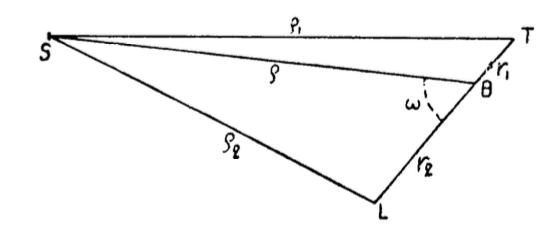
\includegraphics{21.png}
\caption{}\label{21}
\end{figure}

Солнце S сообщает ускорения: 

\begin{table}[bhtp]
    \centering
    \begin{tabular}{c c c r}
        Земле:  $f \cdot \cfrac{S}{\rho_1^2}$ & по & направлению & TS \\[4mm]
        Луне:  $f \cdot \cfrac{S}{\rho_2^2}$ & >> & >> & LS
    \end{tabular}
\end{table} 

\noindent вследствие чего точка $\Theta$ имеет ускорения:

\begin{table}[bhtp]
    \centering
    \begin{tabular}{c c c c r}
        $\cfrac{T}{T + L} \cdot f \cdot \cfrac{S}{\rho_1^2}$ & по & направлению, & параллельному & TS \\[4mm]
        $\cfrac{L}{T + L} \cdot f \cdot \cfrac{S}{\rho_2^2}$ & >> & >> & >> & LS
    \end{tabular}
\end{table}
Ускорения Солнца, происходящие от притяжения Земли и Луны, соответственно, суть:\\
\begin{table}[bhtp]
    \centering
    \begin{tabular}{l c c r}
        $f \cdot \cfrac{T}{\rho_1^2}$ & по & направлению & ST \\[4mm]
        $f \cdot \cfrac{L}{\rho_2^2}$ & >> & >> & SL 
    \end{tabular}
\end{table}

\noindent поэтому ускорения точки $\Theta$ относительно точки $S$ будут:

\begin{table}[bhtp]
    \centering
    \begin{tabular}{l c c c r}
        $\omega_1 = f \cdot \cfrac{\left(S+T+L\right)}{T+L} \cdot \cfrac{T}{\rho_1^2}$ & по & направлению & параллельно & TS \\[4mm]
        $\omega_2 = f \cdot \cfrac{S+T+L}{T+L} \cdot \cfrac{L}{\rho_2^2}$ & >> & >> & >> & LS 
    \end{tabular}
\end{table}

Разлагая эти ускорения, соответственно, по направлениям $\Theta S$ и $\Theta L$, получим, как легко видеть из подобия показанных на рис. \ref{22} и рис. \ref{23} треугольников:

\begin{longtable}{l c c r}
	$\omega_{1}' = \omega_1 \cdot \cfrac{\rho}{\rho_1}$ & по & направлению & $\Theta S$ \\
    $\omega_{1}'' = \omega_1 \cdot \cfrac{r_1}{\rho_1}$ & >> & >> & $\Theta L$ \\ 
    $\omega_{2}' = \omega_2 \cdot \cfrac{\rho}{\rho_2}$ & >> & >> & $\Theta S$ \\
    $\omega_{2}'' = \omega_2 \cdot \cfrac{r_2}{\rho_2}$ & >> & >> & $L\Theta$
\end{longtable}

\begin{wrapfigure}{l}{0.6\linewidth}
    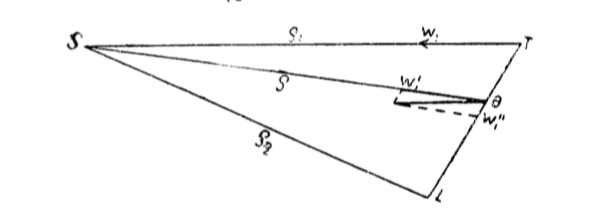
\includegraphics[width=\linewidth, height=2.5cm]{22.png}
	\caption{}\label{22}
\end{wrapfigure}\noindent получим для ускорений точки $\Theta$ слагающие:
\begin{multline}
    W_1 = \omega_{1}' + \omega_{2}' = f \cdot \frac{S+T+L}{T+L}\cdot \\
    \cdot \left[T \cdot \frac{\rho}{\rho_1^3}+L \cdot \frac{\rho}{\rho_2^3} \right] \mbox{ по $\Theta$S} \\    
\end{multline} \\

\begin{equation*}
 W_2 = \omega_{1}'' - \omega_{2}'' = f \cdot \frac{S+T+L}{T+L}\cdot \left[T \cdot \frac{r_1}{\rho_1^3}-L \cdot \frac{r_2}{\rho_2^3} \right] \mbox{ по $\Theta$L}   
\end{equation*}

\begin{figure}[bhtp]
\centering
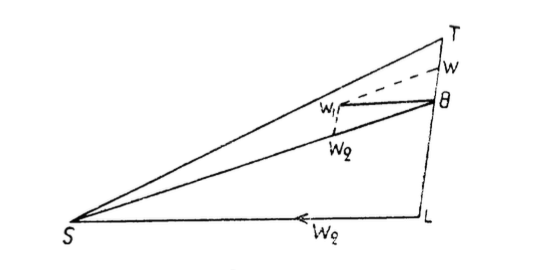
\includegraphics{23.png}
\caption{}\label{23}
\end{figure}

Заменив $r_1$ и $r_2$ их выражениями \eqref{eq:1}, имеем:
\[ W_1 = f \cdot \frac{S+T+L}{T+L} \cdot \rho \cdot \left[ \frac{T}{\rho_1^3} + \frac{L}{\rho_2^3} \right] \mbox{ по направлению $\Theta$S} \] 
\[ W_2 = f \cdot \frac{S+T+L}{\left(T+L\right)^2} \cdot T \cdot L \cdot r  \left[ \frac{1}{\rho_1^3} - \frac{1}{\rho_2^3} \right] \mbox{ по направлению $\Theta$L} \]
\noindent Но:
\[ \rho_1^2 = \rho^2 + 2\rho \cdot \frac{L}{T+L} \cdot r \cos{\omega} + \left(\frac{L}{T+L} \cdot r \right)^2 \] \\
\[ \rho_2^2 = \rho^2 - 2\rho \cdot \frac{T}{T+L} \cdot r \cos{\omega} + \left(\frac{T}{T+L} r \right)^2 \]

\noindent следовательно:
\[ \frac{1}{\rho_1^3} = \frac{1}{\rho^3} \left[ 1+3\frac{L}{T+L}\cos{\omega} + \left(\frac{L}{T+L} r\right)^2\left(-\frac{3}{2} + \frac{15}{2}\cos^2{\omega} \right) + \ldots\right]\]
\[ \frac{1}{\rho_2^3} = \frac{1}{\rho^3} \left[ 1+3\frac{T}{T+L}\cos{\omega} + \left(\frac{T}{T+L} r\right)^2\left(-\frac{3}{2} + \frac{15}{2}\cos^2{\omega} \right) + \ldots\right]\]
Подставляя эти выражения, имеем:
\[ W_1 = f \cdot \frac{S+T+L}{\rho^2} \left[1+\frac{T \cdot L}{\left( T + L \right)^2} \cdot \frac{r^2}{\rho^2} \left(-\frac{3}{2} + \frac{15}{2} \cos^2{\omega} \right) + \ldots \right] \]
\[ W_2 = f \cdot \frac{S+T+L}{\rho^2} \left[-3\cdot\frac{T \cdot L}{\left( T + L \right)^2} \cdot \frac{r^2}{\rho^2} \cos{\omega} + \ldots \right] \]
Но отношения
\[ \frac{L}{T+L} \approx \frac{1}{80}; \; \frac{r}{\rho} \approx \frac{1}{400}; \; \left( \frac{r}{\rho} \right)^2 = \frac{1}{160000} \]
поэтому будет
\[ \frac{T \cdot L}{\left(T+L\right)^2} \cdot \frac{r^2}{\rho^2} \approx \frac{1}{12800000}\]
и члены, содержащие этот множитель, могут быть отброшены, так что будет:
\[ W_1 = f \cdot \frac{S+T+L}{\rho^2} \mbox{ по направлению $\Theta$S} \]
\[ W_2 = 0 \mbox{ по направлению $\Theta$L} \]

Отсюда следует, что точка $\Theta$ движется вокруг Солнца по эллиптической орбите по законам Кеплера. 

Рассмотрим теперь ускорение Луны по отношению к Земле, для чего к ускорениям, сообщаемым Луне Солнцем и Землею, надо присовокупить ускорение, равное и противоположное ускорению Земли, происходящему от действия Солнца и Луны. Поступив подобно предыдущему, получим:
\[ f \cdot \frac{T+L}{r^2}+f \cdot S \left[ \frac{r_2}{\rho_2^3} + \frac{r_1}{\rho_1^3} \right] \mbox{ по направлению L$\Theta$} \]
\[ f \cdot S \cdot \rho \left[ \frac{1}{\rho_2^3} - \frac{1}{\rho_1^3} \right] \mbox{ параллельно $\Theta$S} \]
положим:
\[ T + L = \mu; \; S = M \]

\listoffigures

\listoftables

\end{document}